\section{Tricks in Neural Network}
\label{sec:Solution}
Training neural network to achieve a decent performance in ordinary method
is challenging. In recent years, a growing number of ultra deep neural 
networks, like VGG-16 with 16 layers and over 100 million parameters, 
can be easily trained. The huge leap attributes to the diligent theorists
who devised various sophisticated tricks boosting the training efficiency
and addressing some of the problems mentioned in \autoref{sec:Problem}. 

\subsection{A Good Initialization is All You Need \protect\footnote{The 
title of this section is quoted from Mishkin et al. \parencite{mishkin2015all} whose
title had a profound influence on our study of the neural network.}}

From the experience in \autoref{sssec:Saddle}, a initialization with common 
Gaussian distribution appears to an obstacle to convergence. Romero et al.
\parencite{romero2014fitnets} states that for deep neural net with too many 
layers and especially those with uniform normalization, it is hard to train 
using BP. Thus, we hereby conclude a number of effective initialization methods.

\subsubsection{Xavier Initialization}
In \parencite{glorot2010understanding}, Glorot et al. proposed a adoption of standard
Gaussian initialization which was called "Xavier" initialization by Jia et al.
\parencite{jia2014caffe}. Xavier initialization aims to improve the performance of 
neural network using sigmoid activation and log-likelihood loss function:
\begin{equation}
    \label{equ:Xavier}
    \begin{split}
        E(W^{[l]}) & = 0, \\
        Var(W^{[l]}) & = \frac{2}{n^{[l-1]} - n^{[l]}}
    \end{split}
\end{equation}

\begin{prf}
    For a activation function $ g $ with $ f'(0) = 1 $, like sigmoid $ \sigma(z) $,
    if we use the notation in \autoref{equ:FP} and \autoref{equ:BP}:
    \begin{align*}
        Z^{[l]} & = W^{[l]}A^{[l-1]} + b^{[l]} \\
        dZ^{[l]} & = (W^{[l]T}dZ^{[l+1]})*g^{[l]'}(Z^{[l]}) \\
        dW^{[l]} & = dZ^{[l]}A^{[l-1]T}
    \end{align*} 
    We assume that the weights are independent and the distribution of 
    input $ X $ are the same. Then $ g^{[l]'}(Z_k^{l}) \approx 1 $, Using the 
    chain rule we have:
    \begin{align}
        Var(A^{[l]}) & = Var(X)\prod\limits_{l'=0}^{l-1}n^{[l'-1]}Var(W^{[l']}) \\
        Var(dZ^{[l]}) & = Var(dZ^{[L]})\prod\limits_{l'=L}^{l}n^{[l']}Var(W^{[l']})
    \end{align}
    To keep information flowing in FP and BP, we would like to have:
    \begin{align}
        & \forall(l,\ l'),\ Var(A^{[l]}) = Var(A^{[l']}) \\
        & \forall(l,\ l'),\ Var(dZ^{[l]}) = Var(dZ^{[l']})
    \end{align}
    So:
    \begin{align}
        & \forall l,\ n^{[l'-1]}Var(W^{[l']}) = 1 \\
        & \forall l,\ n^{[l']}Var(W^{[l']}) = 1
    \end{align}
    To combine the two equations above, we may have:
    \begin{eqnarray}
        Var(W^{[l']}) = \frac{2}{n^{[l-1]} - n^{[l]}}
    \end{eqnarray}
    \textbf{Q.E.D.}
\end{prf}
\par For Gaussian initialization, Xavier suggest to have:
\begin{equation}
    W \sim N(0,\ \frac{2}{n^{[l-1]} - n^{[l]}})
\end{equation}
Though rarely in use, a normalized version of Xavier initialization is 
provided in \parencite{glorot2010understanding}:
\begin{equation}
    W \sim U(-\frac{\sqrt{6}}{\sqrt{n^{[l-1]} + n^{[l]}}},\ \frac{\sqrt{6}}{\sqrt{n^{[l-1]} + n^{[l]}}})
\end{equation}

\subsubsection{Kaiming Initialization}
\label{sssec:Kaiming}
He et al. \parencite{he2015delving} extended the \autoref{equ:Xavier} to ReLU
activation and achieved a better performance. In this article, a modification
of ReLU, the Parametric Rectified Linear Unit (PReLU)\footnote{The detail of 
PReLU will be discuss in Appendix 2 } was proposed as well. 
Due to the lack of $ g'(0) = 1 $ in ReLU, "Xavier" failed to pursue a convergence
in deep neural networks. Kaiming initialization is set as follow:
\begin{equation}
    \label{equ:Kaiming}
    \begin{split}
        E(W^{[l]}) & = 0, \\
        Var(W^{[l]}) & = \frac{2}{n^{[l]}}
    \end{split}
\end{equation}

\begin{prf}
    We use the notation in \autoref{equ:FP} and \autoref{equ:BP}:
    \begin{align*}
        Z^{[l]} & = W^{[l]}A^{[l-1]} + b^{[l]} \\
        dA^{[l]} & = W^{[l]T}dZ^{[l+1]}
    \end{align*} 
    And we review the ReLU: $ g(z) = max(0,\ z) $.
    Let the initialization in parameters and input are mutually independent 
    and share the same distribution. Then we have:
    \begin{equation}
        \label{equ:Var}
        \begin{split}
            Var(Z^{[l]}) & = n^{[l]}Var(W^{[l]}A^{[l-1]}) \\
            & = n^{[l]}(Var(W^{[l]})Var(A^{[l-1]}) + Var(W^{[l]})E(A^{[l-1]}))
        \end{split}
    \end{equation}
    Note that $ g(z) = max(0,\ z) $, this leads to $ E(g(z)) = \frac{1}{2}E(z),\ 
    Var(g(z)) = \frac{1}{4}Var(z) $. Therefore, \autoref{equ:Var} can be converted
    to:
    \begin{equation}
        Var(Z^{[l]}) = \frac{1}{2}n^{[l]}Var(W^{[l]})Var(Z^{[l-1]})
    \end{equation}
    Putting all layers together, we have:
    \begin{equation}
        Var(Z^{[L]}) = Var(Z^{1})\prod\limits_{l=2}^L\frac{1}{2}n^{[l]}Var(W^{[l]})
    \end{equation}
    Similar to the proof in Xavier initialization, we hope the maintain the 
    variance in the FP to avoid the possible explosion or vanishing.
    So, 
    \begin{equation}
        \label{equ:Kaiming_1}
        \forall l,\ \frac{1}{2}n^{[l]}Var(W^{[l]}) = 1
    \end{equation}
    Likewise in the process of BP, due to the property of ReLU function, 
    \begin{equation}
        Var(dA^{[1]}) = Var(dA^{L})\prod\limits_{l=1}^L\frac{1}{2}n^{[l]}Var(W^{[l]})
    \end{equation}
    and the corresponding condition is the same as \autoref{equ:Kaiming_1}.
    \textbf{Q.E.D.}
\end{prf}

\subsubsection{Orthogonal Initialization}
Based on deep linear neural networks, Saxe et al. \parencite{saxe2013exact} 
exhibits a class of random orthogonal initialization which enjoys depth 
independent learning time in linear networks. Orthogonal initialization is 
implemented by choosing all weights to be orthogonal matrix:
\begin{equation}
    (W^{[l]})^TW^{[l]} = I
\end{equation}
The implementation can be divided into two steps:
\begin{enumerate}
    \item[1.] Fill the weights with standard Gaussian distribution.
    \item[2.] Decompose the weights matrix using singular value decomposition 
    (SVD) and replace weights with one of the components. 
\end{enumerate}
Saxe et al. suggest that an approriate condition on weights for generating fast
learning speed would be dynamical isometry\footnote{Dynamical isometry means 
that the input-output Jacobian $ J = \frac{\nabla A^{[L]}}{\nabla A^{[0]}} $ 
has all singular values close to 1.}. Saxe et al. \parencite{saxe2013exact} 
illustrate the answer for depth independence by visualize the eigenvalue 
spectrum of a random orthogonal matrix in \autoref{fig:orthogonal}, which is 
exactly a unit circle. Moreover, its singular values are all exactly 1.
\begin{figure}[H]
    \centering
    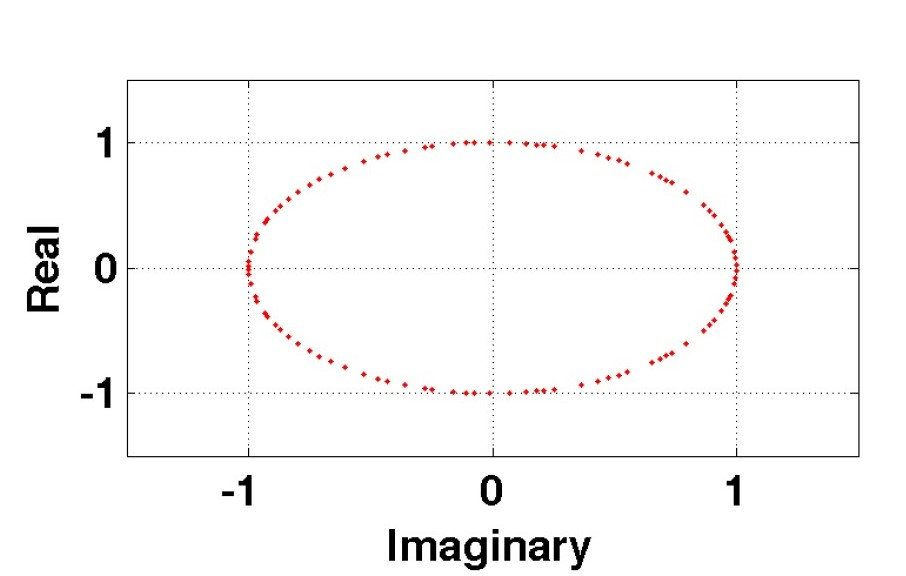
\includegraphics[width=10cm]{orthogonal}
    \caption{\label{fig:orthogonal}The eigenvalue spectrum of a 
    random orthogonal matrix $ W \in \mathbb{R}^{100\times 100} $}
\end{figure}
Then in the linear neural networks, the input-output Jacobian is:
\begin{equation}
    J = \prod\limits_{l=1}^LW^{[l]}
\end{equation}
Under orthogonal initialization in each layer, $ J $ is a orthogonal matrix and
thus the initialization achieve dynamical isometry. Still the reason for dynamical
isometry explaining the depth independence will be studied in the future work.

\subsubsection{Layer-Sequential Unit-Variance Initialization (LSUV)}
As far as we aware, part from the Kaiming initialization, mentioned in 
\autoref{sssec:Kaiming}, there is no extension of Xavier initialization to 
other nonlinear function other than ReLU. Mishkin et al. \parencite{mishkin2015all}
provide a general and simple initialization method that works well with different 
activation functions:
\begin{enumerate}
    \item[1.] Initialize the weights using orthogonal initialization.
    \item[2.] Scale the variance of output of each layer for each mini-batch 
    \footnote{Mini-batch means a small proportion of the data set used in one 
    iteration, which will be introduced in \autoref{sssec:MiniBatch}.} to  
    be 1.
\end{enumerate}
Though the explanation of why LSUV outperform other initialization methods is
not given in the article, a series of comparison empirically show its advantage
in neural networks initialization problem.


\subsection{Gradient Descend Variants}
There are two variants of GD improving the training efficiency. In brevity,
batch describes the data set used in an iteration\footnote{In an iteration, 
all parameters are updated.}, epoch describes a traversal through the whole 
data set. GD introduced in \autoref{ssec:GD} is the basic form of GD. If 
we unroll the vectorization in \autoref{equ:GD}, we can have:
\begin{equation}
    \begin{split}
        dW^{[l]} & = \frac{1}{m}\sum\limits_{i=1}^mdZ_{\bullet,\ i}^{[l]}A_{\bullet,\ i}^{[l-1]T} \\
        db^{[l]} & = \frac{1}{m}\sum\limits_{i=1}^mdZ_{\bullet,\ i}^{[l]}
    \end{split}
\end{equation}  
The variants take on different convergence speed and accuracy by choosing 
different $ m $.

\subsubsection{Batch Gradient Descent (BGD)}
Batch gradient descent, computes the gradient for the whole data set, i.e. 
$ m $ is the size of the data set $ M $. Despite the high accuracy resulted 
from taking full advantage of data set, BGD failed to 
manage the online algorithms due to the considerable training time.

\subsubsection{Stochastic Gradient Descent (SGD)}
In comparison to BGD, SGD is competent for computation
new data on the fly. In each iteration, SGD updates the parameters using
only one piece of data $ (x^{(i)},\ y^{(i)}) $, i.e. $ m = 1 $:
\begin{equation}
    \begin{split}
        dW^{[l]} & = \sum\limits_{i=1}^mdZ^{[l]}A^{[l-1]T} \\
        db^{[l]} & = \sum\limits_{i=1}^mdZ^{[l]} \\
        dZ^{[l]},&\ A^{[l]} \in \mathbb{R}^{n^{[l]}\times 1}
    \end{split}
\end{equation} 
Since only one sample is applied to the computation of gradient, the speed
of SGD is fast enough for daily application. On the other hand, optimizing
for one sample does not guarantee the convergence to a minimum and a descent
of cost in each iteration. It is therefore SGD suffers a severe fluctuation
and may wander around the minimum.

\subsubsection{Mini-batch Gradient Descent (MGD)}
\label{sssec:MiniBatch}
To balance the merit of both BGD and SGD, mini-batch gradient descent
choose an appropriate $ m = 2^k,\ k\in R^+ $. Usually, $ m $ will be chosen
as 64, 128 and 256. Taking the best of both worlds, MGD
descent has a fast and stable convergence.


\subsubsection{Comparison Between Variants}
To illustrate the different between batch BGD, SGD and MGD, we 
implement a multi-classification neural network based on the tensorflow 
framework. The architecture 
of deep neural network with two hidden layers using ReLU and the output 
layer using Softmax, Adam optimization mentioned in \autoref{sssec:Adam} 
is applied to pursue better convergence. Due to the limitation of the 
old version of tensorflow, only Xavier initialization is available.
The code attached in the \" /code/test.py \".
The size of data set is $ M = 1080 $, we set $ m = 1080,\ 1,\ 
64 $ respectively for three variants. The results are shown in the following
, see \autoref{fig:BGD_cost},\autoref{fig:BGD},\autoref{fig:SGD_cost},\autoref{fig:SGD},\autoref{fig:MGD_cost},\autoref{fig:MGD}.

\begin{figure}[H]
    \centering
    \includegraphics[width=8cm]{BGD_cost}
    \caption{\label{fig:BGD_cost}The loss of BGD during training}
\end{figure}

\begin{figure}[H]
    \centering
    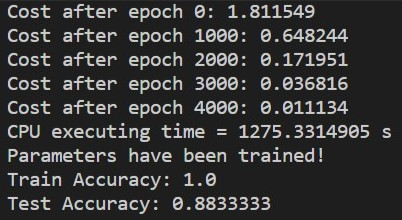
\includegraphics[width=5cm]{BGD}
    \caption{\label{fig:BGD}The result of training}
\end{figure}

\begin{figure}[H]
    \centering
    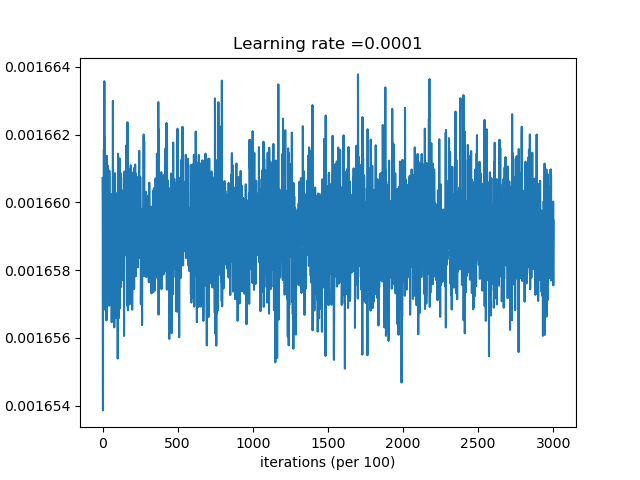
\includegraphics[width=8cm]{SGD_cost}
    \caption{\label{fig:SGD_cost}The loss of SGD during training}
\end{figure}

\begin{figure}[H]
    \centering
    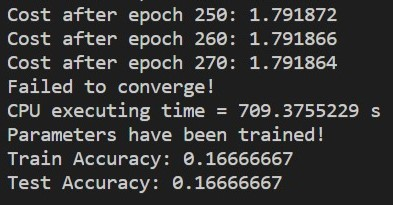
\includegraphics[width=5cm]{SGD}
    \caption{\label{fig:SGD}The result of training}
\end{figure}

\begin{figure}[H]
    \centering
    \includegraphics[width=8cm]{MGD_cost}
    \caption{\label{fig:MGD_cost}The loss of MGD during training}
\end{figure}

\begin{figure}[H]
    \centering
    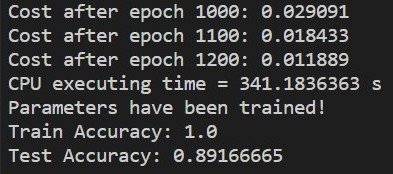
\includegraphics[width=5cm]{MGD}
    \caption{\label{fig:MGD}The result of training}
\end{figure}

\par Unfortunately, under the testing condition, SGD did not converge but stuck
in some kind of local minimum or saddle point. Comparing MGD and BGD, to 
achieve the same accuracy of 99\%, MGD is much more faster but some glitches 
can be observed in the cost, which means MGD dose not guarantee descent in each
iteration like SGD. In all, the simple comparison roughly demonstrate the advantage 
of MGD in the optimization process.


\subsection{Optimization Algorithms}
Mini-batch GD does improve the convergence speed in deep neural
networks, but the aforementioned challenges like saddle points,
learning rate selection are still need to be addressed. We 
summarize some prevailing optimization algorithms as follow.

\subsubsection{Momentum}
Momentum method is one of the earliest simple and robust modification to
pursue faster learning by Qian et al. \parencite{qian1999momentum}. 
When the cost function is similar to a long and 
narrow valley like \autoref{fig:valley}, most gradient is perpendicular
to the long axis, the the back and forth track would drastically slows 
down the learning speed. 

\begin{figure}[H]
    \centering
    \subfigure[Without momentum]{
        \begin{minipage}[t]{0.5\linewidth}
        \centering
        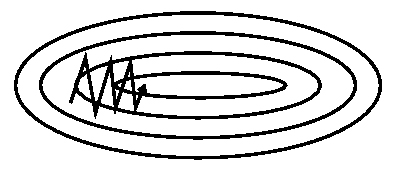
\includegraphics[width=6cm]{Momentum1}
        \end{minipage}%
    }%
    \subfigure[With momentum]{
        \begin{minipage}[t]{0.5\linewidth}
        \centering
        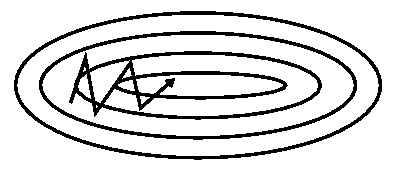
\includegraphics[width=6cm]{Momentum2}
        \end{minipage}%
    }%
    \centering
    \caption{\label{fig:valley}A long and narrow valley 
    situation. From \parencite{momentum}}
\end{figure}

In this situation, we are eager to keep the track
parallel to the long axis by some kind of force. In physics, it is called
the momentum, and thus the terminology comes into being. Momentum updates
the parameters in the following way:
\begin{equation}
    \label{equ:Momentum}
    \begin{split}
        v_{t} & = \beta v_{t-1} - \alpha dW_t^{[l]},\ v_0 = 0 \\
        W_t^{[l]} & = W_{t-1}^{[l]} + v_{t}
    \end{split}
\end{equation}
The recursive definition of $ v_t $ is called the exponentially decaying average.
\par The relation between momentum method and its physics background is readily
comprehensible. When a ball moving in a field with
a fraction w.r.t. the speed, then the Newtonian equation is:
\begin{equation}
    \label{equ:Newton}
    m\frac{d^2x}{dt^2} + \mu\frac{dx}{dt} = -\nabla E(x)
\end{equation}
where $ m $ is the mass, $ \mu $ is the fraction coefficient and $ E(x) $
is the potential energy. Since 
$ \frac{dx}{dt} = \frac{x_{t+1} - x_{t}}{\Delta t} $, \autoref{equ:Newton}
can be rewritten as:
\begin{equation}
    \label{equ:physics}
    \begin{split}
        m\frac{(x_{t+1} - x_{t}) - (x_{t} - x_{t-1})}{(\Delta t)^2} + \mu\frac{x_{t+1} - x_{t}}{\Delta t} = -\nabla E(x) \\
        x_{t+1} - x_{t} = -\frac{(\Delta t)^2}{m+\mu\Delta t}\nabla E(x) + \frac{m}{m+\mu\Delta t}(x_{t} - x_{t-1})
    \end{split}
\end{equation}
If we set $ \frac{(\Delta t)^2}{m+\mu\Delta t} = \alpha,\ 
\frac{m}{m+\mu\Delta t} = \beta $, then we obtain the \autoref{equ:Momentum}.

Here, we briefly demonstrate the convergence analysis of momentum method.
Using the Hessian $ \nabla E(x_t) = Hx_t $ and similarity transformation 
$ H = Q^TDQ,\ Q^TQ = I $, we can convert \autoref{equ:physics} into: 
\begin{equation}
    \begin{split}
        x_{t+1} & = ((1 + \beta)I -\alpha Q^TDQ)x_t - \beta x_{t-1} \\
        Q^Tx_{t+1} & = (1 + \beta)IQ^Tx_t -\alpha Q^TQ^TDQx_t - \beta Q^Tx_{t-1}
    \end{split}
\end{equation}
We denote $ x_t = x_t' $, then the element-wise equation is:
\begin{equation}
    x_{i,\ t+1}' = ((1+\beta)-\alpha d_i)x_{i,\ t}' - \beta x_{i,\ t-1}'
\end{equation}
Then a matrix representation of this equation is:
\begin{equation}
    \label{equ:linear}
    \begin{split}
        \begin{pmatrix}
            x_{i,\ t}' \\
            x_{i,\ t+1}'
        \end{pmatrix}
        = A_i
        \begin{pmatrix}
            x_{i,\ t-1}'   \\
            x_{i,\ t}'
        \end{pmatrix} \\
        A_i = 
        \begin{pmatrix}
            0 & 1   \\
            -\beta & 1 + \beta - \alpha d_i
        \end{pmatrix}
    \end{split}
\end{equation}
The convergence of momentum is determined by the linear system
in \autoref{equ:linear}. Recall the knowledge in numerical
analysis, a theorem w.r.t. the convergent matrix is stated 
in Theorem 7.17 in Burden et al. \parencite{burden2010numerical}:
\begin{thm}
    $ A $ is a convergent matrix\footnote{We call a matrix A convergent if
    \begin{align}
        \lim _{k \rightarrow \infty}\left(A^{k}\right)_{i j}=0, \quad \text{for each } i=1,2, \ldots, n \text{and } j=1,2, \ldots, n
    \end{align}.}
    $\iff$ the spectrum radius $ \rho(A) $\footnote{Spectrum radius is 
    defined as $ \rho(A) $ = max($|\lambda|$)} 
    satisfies
    \begin{equation}
        \rho(A) < 1
    \end{equation}.
\end{thm}
A proposition given in Appendix B in Qian et al. 
\parencite{qian1999momentum} provide the theoretical
foundation of the convergence.
\begin{pro}
    Let $ \lambda_{i,\ 1},\ \lambda_{i,\ 2} $ are the 
    eigenvalues of $ A_i $. The system in \autoref{equ:linear}
    converges if and only if 
    \begin{equation}
        -1 < \beta < 1,\ 0 < \alpha d_i < 2+2\beta 
    \end{equation}
\end{pro}

\subsubsection{Nesterov Accelerated Gradient (NAG)}
\label{sssec:NAG}
NAG in Nesterov \parencite{nesterov1983method}
is a optimization method solving convex problems with 
convergence rate $ O(1/K^2) $, where $ K $ is the number of iterations.
NAG is virtually similar to momentum method in spite of two differences.
First, learning rate is derived from the Armijo rule with $ \beta = 2,\ 
\sigma = 0.5 $ in \autoref{sssec:Armijo}. The momentum constant $ \beta $
is formulated in a recursive way that $ \beta_t \sim \frac{t+4}{2} $, where 
$ t $ is the index of iteration. Second, a subtle update rule is applied 
in NAG. Considering the fact that the former difference just an additional
condition to guarantee the convexity, such formulation seems trivial in 
the common non-convex optimization. Instead, we manually choose the parameters
$ \beta $ and $ \alpha $ in advanced and focus more on the later aspect:
\begin{equation}
    \begin{split}
        v_t & = \beta v_{t-1} - \alpha\nabla J(W_{t-1} + \beta W_{t-1}),\ v_0 = 0 \\
        W_t & = W_{t-1} +  v_t
    \end{split}
\end{equation}
\par To the best of our knowledge, there have been no attempts to generalize the 
convergence analysis of NAG to non-convex problem. But a empirical experiment
in Sutskever's PhD thesis \parencite{sutskever2013training}. 
\par Intuitively, to comprehend the improvement of NAG, imagine SGD as a ball
rolling downhill (like in the physics background of momentum). In a rough terrain,
blindly rolling with gradient seems to be silly, because there is no forecast 
when the ball suddenly face a upward slope. As shown in \autoref{fig:Nesterov}, 
NAG is more stable than momentum due to the backward correction.

\begin{figure}[H]
    \centering
    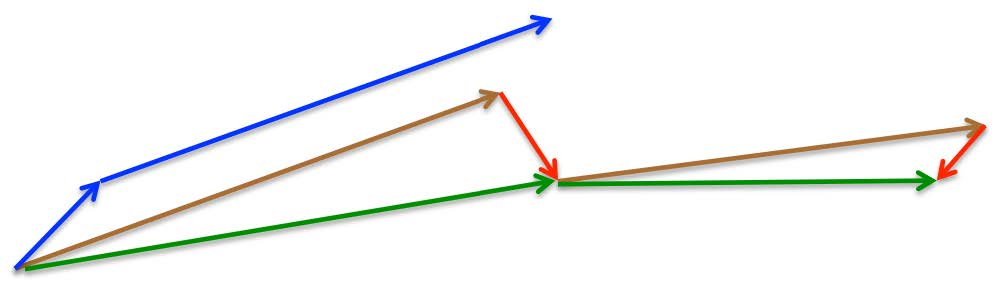
\includegraphics[width=8cm]{Nesterov}
    \caption{\label{fig:Nesterov}NAG illustration: blue vector represents the 
    momentum method, green vector represents the NAG with the brown component 
    is the gradient and the red component is the correction.}
\end{figure}

\subsubsection{RMSprop}
\label{sssec:RMSprop}
It is interesting that RMSprop is not published in paper but propose in a 
Coursera course by Hinton et al. \parencite{rmsprop}. RMSprop adopts the idea
of only using the sign of the gradient by dividing the gradient with the size 
of it:
\begin{equation}
    \begin{split}
        u_t & = \gamma u_{t-1} + (1-\gamma)(dW_t^{[l]})^2,\ u_0 = 0 \\
        W_{t+1}^{[l]} & = W_{t}^{[l]} - \frac{\eta}{\sqrt{u_t+\epsilon}}dW_t^{[l]}
    \end{split}
\end{equation}
Exponentially decaying average $ u_t $ is applied to the second moment of gradient.
In brevity, we denote such average as $ RMS(dW_t^{[l]}) $.
$ \epsilon $ is a smoothing term that prevents division by zero and usually 
set to $ 10^{-8} $. In the lecture, Hinton suggests $ \gamma = 0.9 $.

\subsubsection{Adagrad}
Duchi et al. \parencite{duchi2011adaptive} make a vivid metaphor that some 
infrequent but predictive features are needles in haystacks. Adagrad is a 
subgradient method that crafts domain-specific weightings by performing large
updates for infrequent features and small updates for frequent ones.
\begin{equation}
    W_{t}^{[l]} = W_{t-1}^{[l]} - \frac{\eta}{\sqrt{\sum _{t'=1}^t(dW_{t'}^{[l]})^2} + 
        \epsilon}dW_{t}^{[l]}
\end{equation}
\par Note that the update is divided by the sum of the squared gradients, the 
learning rate will shrink to vanishing with the iteration. To address this flaw,
an adaption called Adadelta is illustrated in the following.

\subsubsection{Adadelta}
Adadelta presented in Zeiler et al. \parencite{zeiler2012adadelta} aims to improve
Adagrad in two aspect: the diminishing learning rate and the manual tunning 
learning rate.
\par First, instead of simply summing up the squared gradients, a accumulation
over window method is introduced, which turns out to be exactly the RMSprop
in \autoref{sssec:RMSprop}. Second, the article suggests that as a 
update of $ W $, $ \Delta W $ should have the same unit as $ W $. However, in usual
optimization method, this is not the case:
\begin{equation}
    \text{units of}\Delta W \propto \text{units of} dW \propto \frac{\partial J}{\partial W} \propto \frac{1}{\text{units of}W}
\end{equation}  
Comparing with the Newton's method in Chapter 10.2 in Burden et al. 
\parencite{burden2010numerical}, the Hessian is used to maintain the same unit:
\begin{equation}
    \Delta W \propto H^{-1} dW \propto \frac{\frac{\partial J}{\partial W}}{\frac{\partial^{2} J}{\partial W^{2}}} \propto \text { units of } W
\end{equation}
The term $ \frac{1}{\frac{\partial^{2} J}{\partial W^{2}}} = \frac{\Delta W}{\frac{\nabla J}{\nabla W}} $
can be added to obtain the match of unit. The unknown $ \Delta W $ in the current iteration
will be substituted by the previous one. Since the denominator use the RMSprop,
the numerator should take the identical form:
\begin{equation}
    \begin{split}
        v_t & = -\frac{RMS(v_{t-1})}{RMS(dW_t^{[l]})} \\
        W_{t+1}^{[l]} & = W_{t}^{[l]} + v_t 
    \end{split}
\end{equation}

\subsubsection{Adam}
\label{sssec:Adam}
The name of Adam comes from adaptive moment estimation in Kingma et al. \parencite{kingma2014adam}
It is a memory saving and easy to compute optimization method combining 
both the advantages of RMSprop and momentum. The pseudo code of Adam is 
shown in \autoref{alg:Adam}.

\begin{algorithm}
    \caption{Adam. Note that all operators are element-wise. The recommended
    hyperparameters are learning rate $ \alpha = 0.001 $, momentum 
    constant $ \beta = 0.9 $, RMSprop constant $ \gamma = 0.999 $, 
    smoothing term $ \epsilon = 10^{-8} $.}
    \label{alg:Adam}
    \begin{algorithmic}
    \REQUIRE $\alpha$: Stepsize
    \REQUIRE $\beta,\ \gamma \in [0,\ 1)]$: Exponential decay rates 
                for moment estimation
    \REQUIRE $J(W)$: Cost function with parameters $ W $
    \REQUIRE $W_0$: Initial parameter
    \STATE $m_0 \gets 0$ (Initialize \engordnumber{1} moment vector)
    \STATE $v_0 \gets 0$ (Initialize \engordnumber{2} moment vector)
    \STATE $t \gets 0$ (Initialize time step)
    \WHILE{$ W_t $ not converged}
    \STATE $ t \gets t + 1 $ 
    \STATE $ g_t \gets \nabla J(W_{t-1}) $(Get gradients w.r.t. cost function)
    \STATE $ m_t \gets \beta m_{t-1} + (1-\beta)g_t $ (Update biased first moment estimate)
    \STATE $ v_t \gets \gamma v_{t-1} + (1-\gamma)g_t^2 $ (Update biased second moment estimate)
    \STATE $ \hat{m_t} \gets \frac{m_{t-1}}{1-\beta^t}$ (Compute bias-corrected first moment estimate)
    \STATE $ \hat{v_t} \gets \frac{v_{t-1}}{1-\gamma^t} $ (Compute bias-corrected second raw moment estimate)
    \STATE $ W_t \gets W_{t-1} - \alpha \frac{\hat{m_t}}{\sqrt{\hat{v_t}}+\epsilon} $ (Update parameters)
    \ENDWHILE
    \RETURN $ W_t $ (Resulting parameters)
    \end{algorithmic}
\end{algorithm}

Using the definition in mathematical statistic, the Exponential decaying average
calculates the mean and uncentered variance of gradients, i.e. the \engordnumber{1}
moment and the \engordnumber{2} raw moment. Due to the initialization of zero which
is not there actual value, the initialization bias correction. Calculate the
recursive definition of $ m_t $, we can obtain:
\begin{align}
    m_t = \beta^tm_0 + (1-\beta)\sum _{i=1}^t\beta^{t-i}g_i
\end{align}
Initialize $ m_0 = 0 $, and we have:
\begin{equation}
    m_t = (1-\beta)\sum _{i=1}^t\beta^{t-i}g_i
\end{equation}
We want the expectation of $ m_t $ and $ g_t $ is equivalent.
\begin{align}
    E(m_t) & = (1-\beta)\sum _{i=1}^t\beta^{t-i}E(g_t) + \zeta \\
    & = (1-\beta^t)E(g_t) + \zeta
\end{align}
If $ E(g_i) $ does not change with time, then $ \zeta=0 $. Even if $ E(g_i) $
varies, an appropriate $ \beta $ can keep $ \zeta $ involved the past gradients
small. Therefore, adding a $ 1-\beta^t $ in the denominator can correct the bias.
\par A analysis of convergence only for convex cost function is given in the 
article \parencite{kingma2014adam}. Under the definition of regret:
\begin{equation}
    R(T) = \sum _{t=1}^T(J(W_t) - J(W^*)) 
\end{equation}
where $ W^* = \mathop{\arg\min}_{W\in (W_1,\cdots,\ W_T)}\sum _{t=1}^TJ(W) $.
The theorem and proof is too obscure, hence we simply illustrate a corollary
showing the bound of regret.
\begin{cor}
    Assume that the function $J$ has bounded gradients, 
    $ ||\nabla J(W)||_2 \leq G,\ ||\nabla J(W)||_\infty \leq G_\infty,
    \ \forall W $, and distance between any $ W_t $ is bounded, 
    $ ||W_m - W_n||_2 \leq D,\ ||W_m - W_n||_\infty \leq D_\infty,\
    \forall m,\ n \in (1,\cdots,\ T) $. Adam achieve the following 
    guarantee:
    \begin{equation}
        \forall T \geq 1,\ \frac{R(T)}{T} = O(\frac{1}{\sqrt{T}})
    \end{equation} 
\end{cor}
Therefore, the regret bound $ O(\sqrt{T}) $ is obtained.

\subsubsection{AdaMax}
AdaMax is a simple and stable extension of Adam is attached
in the same article \parencite{kingma2014adam}. While $L_2$ Norm
is numerically complex, AdaMax uses $L_p$ Norm for the 
\engordnumber{2} raw moment, and let $ p \rightarrow \infty $:
\begin{equation}
    \label{equ:AdaMax}
    \begin{split}
        v_t & = \gamma^\infty v_{t-1} + (1-\gamma^\infty)g_t^\infty \\
        & = max(\gamma v_{t-1},\ |g_t|)
    \end{split}
\end{equation}
The derivation in \autoref{equ:AdaMax} is similar to $L_\infty$ Norm.
In such adaption, even though the initialization of $ v_0 = 0 $, there
is no need to correct the bias. See \autoref{alg:AdaMax} for a complete 
pseudo code.
\begin{algorithm}
    \caption{AdaMax. Note that all operators are element-wise. The recommended
    hyperparameters are learning rate $ \alpha = 0.002 $, momentum 
    constant $ \beta = 0.9 $, RMSprop constant $ \gamma = 0.999 $, 
    smoothing term $ \epsilon = 10^{-8} $.}
    \label{alg:AdaMax}
    \begin{algorithmic}
    \REQUIRE $\alpha$: Stepsize
    \REQUIRE $\beta,\ \gamma \in [0,\ 1)]$: Exponential decay rates 
                for moment estimation
    \REQUIRE $J(W)$: Cost function with parameters $ W $
    \REQUIRE $W_0$: Initial parameter
    \STATE $m_0 \gets 0$ (Initialize \engordnumber{1} moment vector)
    \STATE $v_0 \gets 0$ (Initialize \engordnumber{2} moment vector)
    \STATE $t \gets 0$ (Initialize time step)
    \WHILE{$ W_t $ not converged}
    \STATE $ t \gets t + 1 $ 
    \STATE $ g_t \gets \nabla J(W_{t-1}) $(Get gradients w.r.t. cost function)
    \STATE $ m_t \gets \beta m_{t-1} + (1-\beta)g_t $ (Update biased first moment estimate)
    \STATE $ v_t \gets max(\gamma v_{t-1},\ |g_t|) $ (Update the exponentially weighted infinity norm)
    \STATE $ \hat{m_t} \gets \frac{m_{t-1}}{1-\beta^t}$ (Compute bias-corrected first moment estimate)
    \STATE $ W_t \gets W_{t-1} - \alpha \frac{\hat{m_t}}{v_t} $ (Update parameters)
    \ENDWHILE
    \RETURN $ W_t $ (Resulting parameters)
    \end{algorithmic}
\end{algorithm}

\subsubsection{NAdam}
NAG in \autoref{sssec:NAG} shows a powerful correction for momentum,  and it is 
generally acknowledged that standard momentum is inferior to NAG. Dozat 
\parencite{dozat2016incorporating} improves Adam's momentum part to NAG and 
achieves faster convergence speed.
\par First, Dozat modifies the NAG by applying a look ahead momentum to the update:
\begin{equation}
    \begin{split}
        v_t & = \beta v_{t-1} - \nabla J(W_{t-1}),\ v_0 = 0 \\
        W_t & = W_{t-1} +  \beta v_t + \alpha \nabla J(W_{t-1})
    \end{split}
\end{equation} 
Then we can modify Adam in the following way:
\begin{equation}
    \begin{split}
        W_t & = W_{t-1} - \alpha \frac{m_t}{(\sqrt{\hat{v_t}} + \epsilon)(1-\beta^t)} \\
        & = W_{t-1} - \alpha \frac{\beta m_t + (1-\beta)g_t}{(\sqrt{\hat{v_t}} + \epsilon)(1-\beta^t)} \\
        & = W_{t-1} - \frac{\alpha}{\sqrt{\hat{v_t}} + \epsilon}(\beta \hat{m_t} + \frac{(1-\beta)g_t}{1-\beta^t})
    \end{split}
\end{equation}
A complete algorithm is shown in \autoref{alg:NAdam}.

\begin{algorithm}[H]
    \caption{NAdam. Note that all operators are element-wise. The recommended
    hyperparameters are learning rate $ \alpha = 0.002 $, momentum 
    constant $ \beta = 0.975 $, RMSprop constant $ \gamma = 0.999 $, 
    smoothing term $ \epsilon = 10^{-8} $.}
    \label{alg:NAdam}
    \begin{algorithmic}
    \REQUIRE $\alpha$: Stepsize
    \REQUIRE $\beta,\ \gamma \in [0,\ 1)]$: Exponential decay rates 
                for moment estimation
    \REQUIRE $J(W)$: Cost function with parameters $ W $
    \REQUIRE $W_0$: Initial parameter
    \STATE $m_0 \gets 0$ (Initialize \engordnumber{1} moment vector)
    \STATE $v_0 \gets 0$ (Initialize \engordnumber{2} moment vector)
    \STATE $t \gets 0$ (Initialize time step)
    \WHILE{$ W_t $ not converged}
    \STATE $ t \gets t + 1 $ 
    \STATE $ g_t \gets \nabla J(W_{t-1}) $(Get gradients w.r.t. cost function)
    \STATE $ m_t \gets \beta m_{t-1} + (1-\beta)g_t $ (Update biased first moment estimate)
    \STATE $ v_t \gets \gamma v_{t-1} + (1-\gamma)g_t^2 $ (Update biased second moment estimate)
    \STATE $ \hat{m_t} \gets \frac{m_{t-1}}{1-\beta^t}$ (Compute bias-corrected first moment estimate)
    \STATE $ \hat{v_t} \gets \frac{v_{t-1}}{1-\gamma^t} $ (Compute bias-corrected second raw moment estimate)
    \STATE $ W_t \gets W_{t-1} - \frac{\alpha}{\sqrt{\hat{v_t}}+\epsilon}(\beta \hat{m_t} + \frac{(1-\beta)g_t}{1-\beta^t}) $ (Update parameters)
    \ENDWHILE
    \RETURN $ W_t $ (Resulting parameters)
    \end{algorithmic}
\end{algorithm}

\begin{comment}
    \subsubsection{Comparison}
\end{comment}